\documentclass[11pt]{article}

\usepackage{amsmath,amssymb,amsthm}
\usepackage{geometry}
\usepackage{enumitem}
\usepackage{mathtools}
\usepackage{hyperref}

\usepackage{tikz}
\usetikzlibrary{arrows.meta,positioning}

\geometry{margin=1in}

\title{Mentis Umbra:\\
Consciousness, Agency, and Qualia as Admissible Projections}

\author{Amos Jay Maley}
\date{}

\theoremstyle{definition}
\newtheorem{definition}{Definition}
\newtheorem{lemma}{Lemma}
\newtheorem{theorem}{Theorem}
\newtheorem{corollary}{Corollary}

\begin{document}
\maketitle

\begin{abstract}
We establish a structural classification theorem: any admissible irreversible system that is redescription-stable must instantiate a projection structure consisting of a transition mediator and an invariant reference. We further extend the result to interacting multi-system cases, proving existence and necessity-under-removal of interaction mediators and jointly invariant references, lifting to $n$-system settings via pairwise restriction, and giving a constructive global mediation criterion via triple compatibility. Terminology relating to agency, intentionality, and interior representation is introduced only as role-based naming conventions for derived structural predicates. No new primitives are introduced.
\end{abstract}

\section{Framework Axioms}
This paper assumes the Core Framework Axioms stated in Appendix~A.
All references to admissibility, standing, and redescription stability are governed by these axioms.


\section{Quotient-Mediator Clarification}

Let $\approx$ denote equivalence under admissible redescription: 
$X \approx Y$ iff $\exists R$ admissible with $R(X)\sim Y$.

Define the canonical projection
\[
\pi: S \to S/{\approx}.
\]

\begin{lemma}[Descent to Quotient]
If redescription stability holds, then for every $T \in E(S)$ there exists a unique induced map
$\widehat{T}$ such that
\[
\pi(T(S)) = \widehat{T}(\pi(S)).
\]
\end{lemma}

\begin{proof}
If $X \approx Y$, then $Y \sim R(X)$ for some admissible $R$.
By redescription stability,
\[
T(Y) \sim T(R(X)) \sim R(T(X)).
\]
Hence $T(X) \approx T(Y)$, so $T$ is constant on $\approx$-classes and descends uniquely.
\end{proof}

This quotient projection provides the canonical mediator structure referenced throughout the paper.


% =========================================================
\section{Single-System Framework (Fully Formal)}

\subsection{Typing/Applicability and Irreversibility}

\begin{definition}[Single-System Envelope]
Let $S$ be a system.
Define $\mathcal{E}(S)$ to be the set of transition operators $T$
such that the application $T(S)$ is well-defined and yields a system of the same structural type as $S$.
This is a typing/applicability domain only; it imposes no semantic condition on transition outcomes.
\end{definition}

\paragraph{Remark (Presentation Regime Dichotomy).}
Statewise envelope non-minimality is a syntactic condition on representation:
it asserts absence of a canonical presentation at each well-typed state.
If a canonicalization discipline were imposed (eliminating all non-identity alpha-variants),
then the non-minimality condition would fail and the determinacy argument would trivialize.
Thus the results bifurcate cleanly between canonical and non-canonical presentation regimes.


\begin{definition}[Irreversible Transition]
A transition $T \in \mathcal{E}(S)$ is \emph{irreversible} if there does not exist any admissible transition
$U \in \mathcal{E}(T(S))$ such that
\[
U(T(S)) \sim S.
\]
\end{definition}

\subsection{Equivalence, Redescription, and Stability}

\begin{definition}[Identity Equivalence]
For systems $S_1,S_2$, we write
\[
S_1 \sim S_2
\]
iff:
\begin{enumerate}[label=(\roman*)]
    \item standing status matches,
    \item $\mathcal{E}(S_1)=\mathcal{E}(S_2)$,
    \item for every $T\in \mathcal{E}(S_1)$, the outcomes $T(S_1)$ and $T(S_2)$ agree up to alpha-equivalence of internal representation symbols only.
\end{enumerate}
No semantic drift beyond alpha-equivalence is permitted.
\end{definition}

\begin{definition}[Admissible Redescription]
A transformation $R$ on system representations is \emph{admissible} if:
\begin{enumerate}[label=(\roman*)]
    \item standing status is preserved,
    \item typing/applicability envelope is preserved:
    \[
    \mathcal{E}(S)=\mathcal{E}(R(S)),
    \]
    \item no anchors are introduced and none are removed,
    \item identity equivalence under $\sim$ is preserved (alpha-equivalence only).
\end{enumerate}
\end{definition}

\begin{definition}[Redescription Stability]
A system $S$ is \emph{redescription-stable} if for every admissible redescription $R$ and every $T\in \mathcal{E}(S)$,
\[
R(T(S)) \sim T(R(S)).
\]
\end{definition}

\subsection{Mediator Factorization and Invariant Reference}

\begin{definition}[Transition Mediator]
A structure $P$ is a \emph{mediator} for $S$ if for every $T \in \mathcal{E}(S)$ there exists an induced operator $\widehat{T}$ such that
\[
T(S)=\widehat{T}(P(S)).
\]
\end{definition}

\begin{lemma}[Nontrivial Admissible Renaming]
If evaluation of some $T\in\mathcal{E}(S)$ depends on internal representation labels beyond
alpha-equivalence, then there exists an admissible redescription $R$ that renames internal symbols while preserving $\sim$.
\end{lemma}

\begin{proof}
Because admissible redescriptions preserve standing, preserve typing envelope, and permit alpha-equivalence only,
any bijective renaming of internal representation symbols that preserves well-typedness and introduces/removes no anchors
is admissible. If evaluation depends on raw labels not quotiented by alpha-equivalence, applying such a renaming changes the
evaluation result while preserving identity equivalence up to alpha-equivalence. Hence such an admissible $R$ exists.
\end{proof}

\begin{lemma}[Mediator Necessity]
Let $S$ be redescription-stable. Then transition semantics factor through some mediator $P$.
\end{lemma}

\begin{proof}
Assume no mediator exists. Then there exists $T\in\mathcal{E}(S)$ such that the evaluation of $T(S)$ depends on internal
representation labels beyond alpha-equivalence (otherwise one can factor through the quotient-by-alpha-equivalence summary of
the required label-invariant information). By the Nontrivial Admissible Renaming Lemma, there exists an admissible redescription
$R$ that renames internal labels while preserving $\sim$. Because $T$ is label-sensitive beyond alpha-equivalence, the two
computations differ beyond alpha-equivalence, so
\[
R(T(S)) \not\sim T(R(S)).
\]
This contradicts redescription stability. Therefore a mediator $P$ must exist.
\end{proof}

\begin{definition}[Invariant Reference Structure]
A reference structure $I$ is \emph{invariant} under admissible redescriptions if for every admissible $R$,
\[
R(I)\sim I.
\]
\end{definition}

\begin{lemma}[Invariant Reference Necessity]
Let $S$ be redescription-stable and let $P$ be a mediator for $S$. Then there exists an invariant reference structure $I$.
\end{lemma}

\begin{proof}
Assume no invariant reference structure exists. Then there exists an admissible redescription $R$ such that any candidate
reference resolution differs under $R$ while preserving alpha-equivalence at the raw representation level.

Because transitions factor through the mediator $P$, consistency of transition composition and identity persistence must be
computed relative to a redescription-invariant reference resolution; otherwise the induced transition operators $\widehat{T}$
cannot be well-defined on identity-equivalence classes under redescription. Concretely, under reference drift there exists
$T\in\mathcal{E}(S)$ whose induced evaluation (via $P$) depends on the choice of reference resolution, yielding
\[
R(T(S)) \not\sim T(R(S)).
\]
This contradicts redescription stability. Therefore an invariant reference structure $I$ must exist.
\end{proof}

\subsection{Single-System Projection Necessity and Necessity-Under-Removal}

\begin{theorem}[Single-System Projection Necessity]
Let $S$ be redescription-stable. Then there exist structures $(P,I)$ such that:
\begin{enumerate}[label=(\roman*)]
    \item for every $T\in\mathcal{E}(S)$, $T(S)=\widehat{T}(P(S))$ for some induced $\widehat{T}$,
    \item for every admissible $R$, $R(I)\sim I$,
    \item identity equivalence is preserved under transition composition (by redescription stability).
\end{enumerate}
\end{theorem}

\begin{proof}
By Lemma (Mediator Necessity), there exists a mediator $P$.
By Lemma (Invariant Reference Necessity), there exists an invariant reference structure $I$.
Redescription stability provides commutation for all $T\in\mathcal{E}(S)$ and admissible $R$, hence preserves identity equivalence
under compositions of well-typed transitions.
\end{proof}

\begin{theorem}[Necessity Under Removal (Single-System)]
If either (a) mediator factorization is absent or (b) invariant reference is absent, then there exist admissible $R$ and
$T\in\mathcal{E}(S)$ such that redescription stability fails:
\[
R(T(S))\not\sim T(R(S)).
\]
\end{theorem}

\begin{proof}
(a) Without mediator factorization, some transition evaluation remains label-sensitive beyond alpha-equivalence, so the Nontrivial
Admissible Renaming Lemma yields an admissible $R$ producing commutation failure for that transition.

(b) Without invariant reference, reference resolution can drift under admissible redescriptions; by the Invariant Reference Necessity
proof, there exists $T$ for which induced evaluation differs beyond alpha-equivalence, producing commutation failure.
\end{proof}

% =========================================================
\section{Role-Based Classification (Non-Primitive Naming)}

\begin{definition}[Agency-Structure Predicate]
For a projection structure $(P,I)$, define $A(P,I)$ to hold if irreversible transitions are evaluated relative to invariant reference $I$.
\end{definition}

\begin{definition}[Intentional-Structure Predicate]
Define $M(P,I)$ to hold if transition evaluation includes state--target resolution mediated through $P$.
\end{definition}

\begin{definition}[Interior-Representation Predicate]
Define $Q(P,I)$ to hold if mediator $P$ provides compressed coordination sufficient for redescription stability.
\end{definition}

\begin{lemma}[Role Predicates Hold for Single-System Projection Structures]
If $(P,I)$ satisfies the Single-System Projection Necessity theorem, then $A(P,I)$, $M(P,I)$, and $Q(P,I)$ hold.
\end{lemma}

\begin{proof}
Factorization through $P$ implies transition evaluation is mediated (hence supports state--target resolution via the induced operators),
and invariance of $I$ implies evaluation is relative to a redescription-invariant reference. The existence of a mediator that blocks
label-sensitivity beyond alpha-equivalence supplies the required compression for stable coordination. Thus $A$, $M$, and $Q$ hold.
\end{proof}

\paragraph{Terminology Convention.}
We refer to $A$ as \emph{agency-structure}, $M$ as \emph{intentional-structure}, and $Q$ as \emph{interior-representation-structure}.
These are role-names only and introduce no new primitives.

% =========================================================

% =========================================================
\section{Illustrative Example (Non-Primitive)}

This section is illustrative only and introduces no new primitives or assumptions.

\subsection{Example: Neural State Transition as Mediated Evaluation}

Consider a biological cognitive system whose internal state transitions are described
at some representational level as neural state updates.

Let $S$ denote the current neural state and let $T \in \mathcal{E}(S)$
represent a well-typed neural transition (e.g., synaptic update under lawful dynamics).

If transition evaluation depended directly on raw neuron labels
rather than label-invariant structure,
then an admissible redescription $R$ (renaming neuron indices
without altering functional organization)
would yield:

\[
R(T(S)) \not\sim T(R(S)),
\]

violating redescription stability.

Therefore transition evaluation must factor through
a mediator $P$ that captures only the label-invariant structural content
required for lawful update.

The invariant reference $I$ corresponds structurally to a stable index
under which successive neural transitions are attributed consistently
across admissible redescriptions.

This example does not introduce neuroscience as a primitive.
It merely instantiates the formal structure in a familiar domain.


\section{Multi-System Interaction (Fully Formal)}

\subsection{Joint Typing, Equivalence, and Stability}

\begin{definition}[Joint System]
Let $S_1,S_2$ be systems. The joint system is
\[
S_{12}:=(S_1,S_2).
\]
\end{definition}

\begin{definition}[Joint Envelope]
Define $\mathcal{E}_{12}(S_{12})$ to be the set of joint transition operators $J$ such that
\[
J(S_{12})=(S_1',S_2')
\]
is well-defined and yields a joint system of the same arity. This is a typing/applicability domain only.
\end{definition}

\begin{definition}[Joint Identity Equivalence]
For joint systems $S_{12}=(S_1,S_2)$ and $S_{12}'=(S_1',S_2')$, write
\[
S_{12}\sim S_{12}'
\]
iff:
\begin{enumerate}[label=(\roman*)]
    \item $S_1\sim S_1'$ and $S_2\sim S_2'$,
    \item standing matches componentwise,
    \item $\mathcal{E}_{12}(S_{12})=\mathcal{E}_{12}(S_{12}')$,
    \item for every $J\in\mathcal{E}_{12}(S_{12})$, the outcomes $J(S_{12})$ and $J(S_{12}')$ agree up to alpha-equivalence only.
\end{enumerate}
No semantic drift beyond alpha-equivalence is permitted.
\end{definition}

\begin{definition}[Admissible Joint Redescription]
A transformation $R_{12}$ on joint representations is admissible if:
\begin{enumerate}[label=(\roman*)]
    \item standing preserved componentwise,
    \item joint envelope preserved:
    \[
    \mathcal{E}_{12}(S_{12})=\mathcal{E}_{12}(R_{12}(S_{12})),
    \]
    \item no anchors introduced or removed,
    \item joint identity equivalence under $\sim$ preserved (alpha-equivalence only).
\end{enumerate}
\end{definition}

\begin{definition}[Joint Redescription Stability]
$S_{12}$ is jointly redescription-stable if for all admissible $R_{12}$ and all $J\in\mathcal{E}_{12}(S_{12})$,
\[
R_{12}(J(S_{12}))\sim J(R_{12}(S_{12})).
\]
\end{definition}

\subsection{Componentwise Closure and Well-Formedness}

\begin{lemma}[Componentwise Closure of Joint Admissibility]
Let $R_1$ be an admissible redescription on $S_1$ and $R_2$ an admissible redescription on $S_2$.
Define
\[
R_{12}(S_{12}) := (R_1(S_1),R_2(S_2)).
\]
Then $R_{12}$ is an admissible joint redescription.
\end{lemma}

\begin{proof}
Standing preservation holds componentwise. Typing preservation of each component implies typing preservation on the ordered pair, hence
the joint envelope is preserved. No anchors are introduced/removed componentwise, hence none jointly. Alpha-equivalence-only identity
preservation holds componentwise and therefore jointly. Thus $R_{12}$ satisfies the admissibility conditions.
\end{proof}

\begin{lemma}[Well-Formedness of Joint Stability]
Let $R_{12}$ be admissible and $J\in\mathcal{E}_{12}(S_{12})$. Then $R_{12}(J(S_{12}))$ and $J(R_{12}(S_{12}))$ are well-defined,
and the stability statement is well-formed.
\end{lemma}

\begin{proof}
Since $J\in\mathcal{E}_{12}(S_{12})$, $J(S_{12})$ is well-defined. Admissible $R_{12}$ preserves typing, hence $R_{12}(J(S_{12}))$ is well-defined.
Envelope preservation implies $J\in\mathcal{E}_{12}(R_{12}(S_{12}))$, hence $J(R_{12}(S_{12}))$ is well-defined. Therefore the relation is well-formed.
\end{proof}

\subsection{Joint Irreversibility and Nontrivial Renaming}

\begin{definition}[Joint Irreversible Transition]
A joint transition $J\in\mathcal{E}_{12}(S_{12})$ is irreversible if there does not exist admissible
$K\in\mathcal{E}_{12}(J(S_{12}))$ such that
\[
K(J(S_{12}))\sim S_{12}.
\]
\end{definition}

\begin{lemma}[Nontrivial Admissible Joint Renaming]
If evaluation of some $J\in\mathcal{E}_{12}(S_{12})$ depends on internal labels beyond alpha-equivalence,
then there exists an admissible joint redescription $R_{12}$ that renames internal symbols while preserving $\sim$.
\end{lemma}

\begin{proof}
As in the single-system case: any bijective renaming preserving well-typedness, standing, and anchors is admissible.
If evaluation depends on raw labels beyond alpha-equivalence, such a renaming changes evaluation while preserving $\sim$.
\end{proof}

\subsection{Joint Mediators and Joint Invariant References}

\begin{definition}[Joint Transition Mediator]
A structure $P_{12}$ is a joint mediator if for every $J\in\mathcal{E}_{12}(S_{12})$ there exists induced $\widehat{J}$ such that
\[
J(S_{12})=\widehat{J}(P_{12}(S_{12})).
\]
\end{definition}

\begin{lemma}[Joint Mediator Necessity]
Let $S_{12}$ be jointly redescription-stable. Then there exists a joint mediator $P_{12}$.
\end{lemma}

\begin{proof}
Assume no joint mediator exists. Then some $J\in\mathcal{E}_{12}(S_{12})$ is label-sensitive beyond alpha-equivalence.
By the Nontrivial Admissible Joint Renaming Lemma, there exists admissible $R_{12}$ renaming internal labels while preserving $\sim$.
Because $J$ is label-sensitive, the two computations differ beyond alpha-equivalence, yielding
\[
R_{12}(J(S_{12}))\not\sim J(R_{12}(S_{12})),
\]
contradicting joint redescription stability. Therefore a joint mediator exists.
\end{proof}

\begin{definition}[Joint Invariant Reference Pair]
A pair $(I_1,I_2)$ is jointly invariant if for every admissible joint redescription $R_{12}$,
\[
R_{12}(I_1,I_2)\sim (I_1,I_2).
\]
\end{definition}

\begin{lemma}[Joint Invariant Reference Necessity]
Let $S_{12}$ be jointly redescription-stable and let $P_{12}$ be a joint mediator. Then there exists a jointly invariant reference pair $(I_1,I_2)$.
\end{lemma}

\begin{proof}
Assume no jointly invariant reference pair exists. Then there exists admissible $R_{12}$ such that reference resolution drifts while preserving
alpha-equivalence at the representation level:
\[
R_{12}(I_1,I_2)\not\sim (I_1,I_2).
\]
Because joint transitions factor through $P_{12}$, stable evaluation under composition requires jointly invariant reference resolution; otherwise the induced
operators cannot be well-defined on joint identity equivalence classes under admissible redescriptions. Therefore there exists
$J\in\mathcal{E}_{12}(S_{12})$ such that induced evaluation differs beyond alpha-equivalence, yielding
\[
R_{12}(J(S_{12}))\not\sim J(R_{12}(S_{12})),
\]
contradicting joint stability. Hence a jointly invariant reference pair exists.
\end{proof}

\subsection{Joint Projection Necessity and Necessity-Under-Removal}

\begin{theorem}[Interaction Projection Necessity (Two-System)]
Let $S_{12}$ be jointly redescription-stable. Then:
\begin{enumerate}[label=(\roman*)]
    \item each component $S_i$ is redescription-stable as a single system under admissible componentwise redescriptions, and thus instantiates $(P_i,I_i)$,
    \item there exists a joint mediator $P_{12}$,
    \item there exists a jointly invariant reference pair $(I_1,I_2)$.
\end{enumerate}
\end{theorem}

\begin{proof}
(i) Let $R_1$ be an admissible redescription on $S_1$ and let $R_2$ be identity on $S_2$. By the Componentwise Closure Lemma, the induced $R_{12}$ is admissible.
Consider a joint transition $J$ that acts as some $T\in\mathcal{E}(S_1)$ on the first component and as identity on the second. Such $J$ is well-typed and in
$\mathcal{E}_{12}(S_{12})$. Joint stability gives
\[
R_{12}(J(S_{12}))\sim J(R_{12}(S_{12})).
\]
Projecting to the first component yields $R_1(T(S_1))\sim T(R_1(S_1))$ for all admissible $R_1$ and all $T\in\mathcal{E}(S_1)$, i.e. $S_1$ is redescription-stable.
Similarly for $S_2$. By the single-system theorems, each component instantiates $(P_i,I_i)$.

(ii) Joint mediator existence is Lemma (Joint Mediator Necessity).

(iii) Joint invariant reference pair existence is Lemma (Joint Invariant Reference Necessity).
\end{proof}

\begin{theorem}[Necessity Under Removal (Joint)]
If either (a) joint mediator factorization is absent or (b) joint invariant reference fails, then there exist admissible $R_{12}$ and $J\in\mathcal{E}_{12}(S_{12})$
such that joint redescription stability fails:
\[
R_{12}(J(S_{12}))\not\sim J(R_{12}(S_{12})).
\]
\end{theorem}

\begin{proof}
(a) Without mediator factorization, some joint transition evaluation remains label-sensitive beyond alpha-equivalence, so the Nontrivial Admissible Joint Renaming Lemma
yields an admissible $R_{12}$ producing commutation failure.

(b) Without joint invariant reference, reference resolution can drift under admissible joint redescriptions; by the Joint Invariant Reference Necessity proof, there exists
$J$ producing commutation failure.
\end{proof}

% =========================================================
\section{Extension to $n$ Systems (Fully Formal)}

\subsection{Restriction Maps and Restricted Actions}

\begin{definition}[Pairwise Restriction and Inclusion]
Let $S_{1\ldots n}=(S_1,\ldots,S_n)$ be a joint system. For indices $i\neq j$, define
\[
\pi_{ij}(S_{1\ldots n}) := (S_i,S_j)=:S_{ij}.
\]
Define the inclusion map $\iota_{ij}$ from $S_{ij}$ into $S_{1\ldots n}$ by holding all components other than $i,j$ fixed.
\end{definition}

\begin{definition}[Restricted Redescription]
Let $R_{1\ldots n}$ be a joint redescription on $S_{1\ldots n}$. Define its restriction to $(i,j)$ by
\[
R_{ij} := \pi_{ij}\circ R_{1\ldots n}\circ \iota_{ij},
\]
whenever well-typed.
\end{definition}

\begin{definition}[Restricted Joint Transition]
Let $J_{1\ldots n}$ be a joint transition on $S_{1\ldots n}$. If $J_{1\ldots n}$ acts nontrivially only on components $(i,j)$ and as identity on all others,
define its restriction $J_{ij}$ by
\[
J_{ij}(S_{ij}) := \pi_{ij}\!\left(J_{1\ldots n}(\iota_{ij}(S_{ij}))\right).
\]
\end{definition}

\subsection{Inherited Pairwise Stability}

\begin{lemma}[Inherited Pairwise Stability]
Assume $S_{1\ldots n}$ is jointly redescription-stable (in the natural $n$-system extension).
Fix $i\neq j$. Then the pairwise subsystem $S_{ij}$ is jointly redescription-stable under admissible restricted redescriptions and well-typed restricted transitions:
\[
R_{ij}(J_{ij}(S_{ij}))\sim J_{ij}(R_{ij}(S_{ij})).
\]
\end{lemma}

\begin{proof}
Let $R_{ij}$ be any admissible redescription on $S_{ij}$. Extend it to an admissible $R_{1\ldots n}$ that acts as $R_{ij}$ on components $(i,j)$ and as identity on all others.
Let $J_{ij}$ be any well-typed joint transition on $S_{ij}$ and extend it to $J_{1\ldots n}$ acting as $J_{ij}$ on $(i,j)$ and as identity on all other components.
Apply joint stability of $S_{1\ldots n}$ to $R_{1\ldots n}$ and $J_{1\ldots n}$, then restrict both sides by $\pi_{ij}$. Typing preservation and alpha-equivalence-only
equivalence ensure the restricted commutation holds.
\end{proof}

\begin{corollary}[Forced Pairwise Interaction Structures]
If $S_{1\ldots n}$ is jointly redescription-stable, then for every pair $(i,j)$ the subsystem $S_{ij}$ instantiates a joint mediator $P_{ij}$ and jointly invariant references $(I_i,I_j)$.
\end{corollary}

% =========================================================
\section{Constructive Global Mediation and Compatibility}

\subsection{Product Mediator Construction}

Assume $S_{1\ldots n}$ is jointly redescription-stable. By the previous corollary, for each pair $(i,j)$ a joint mediator $P_{ij}$ exists.

\begin{definition}[Product Mediator]
Define the product mediator $P^{\Pi}_{1\ldots n}$ by
\[
P^{\Pi}_{1\ldots n}(S_{1\ldots n})
:=
\bigl(P_{ij}(\pi_{ij}(S_{1\ldots n}))\bigr)_{1\le i<j\le n}.
\]
\end{definition}

\subsection{Triple Compatibility}

\begin{definition}[Triple Compatibility (Consistency Constraint)]
The family $\{P_{ij}\}$ is triple-compatible if for all distinct $i,j,k$ and all states $S_{1\ldots n}$, the induced pairwise mediator outputs agree on overlaps up to $\sim$,
i.e., whenever well-typed,
\[
P_{ij}(\pi_{ij}(S_{1\ldots n})) \sim \pi_{ij}\!\left(P_{ik}(\pi_{ik}(S_{1\ldots n}))\right),
\]
and similarly with $(ik)$ replaced by $(jk)$.
\end{definition}


\subsection{Pairwise Determinacy Forced by Stability}

\begin{definition}[Pairwise Indistinguishability]
For joint states $X,Y$ of $S_{1\ldots n}$, write
\[
X \equiv_{\Pi} Y
\]
iff their product mediator values agree up to $\sim$, i.e.
\[
P^{\Pi}_{1\ldots n}(X) \sim P^{\Pi}_{1\ldots n}(Y),
\]
meaning each pairwise component satisfies
\[
P_{ij}(\pi_{ij}(X)) \sim P_{ij}(\pi_{ij}(Y))
\quad\text{for all } i<j.
\]
\end{definition}

\begin{definition}[Pairwise-Preserving Renaming]
An admissible joint redescription $R_{1\ldots n}$ is a \emph{pairwise-preserving renaming} if:
\begin{enumerate}[label=(\roman*)]
    \item $R_{1\ldots n}$ is an admissible joint redescription,
    \item $R_{1\ldots n}$ acts as a pure alpha-renaming on internal representation symbols (no semantic drift),
    \item for all joint states $X$,
    \[
    P^{\Pi}_{1\ldots n}(R_{1\ldots n}(X)) \sim P^{\Pi}_{1\ldots n}(X).
    \]
\end{enumerate}
\end{definition}

\begin{lemma}[Renaming Invariance of Identity Equivalence]
If $R$ is an admissible redescription that is a pure alpha-renaming, then for every well-typed state $Z$,
\[
R(Z) \sim Z.
\]
\end{lemma}

\begin{proof}
By definition, a pure alpha-renaming preserves standing, preserves typing, introduces/removes no anchors, and changes only symbol names.
Identity equivalence $\sim$ permits alpha-equivalence only, and forbids semantic drift beyond alpha-equivalence. Therefore $R(Z)\sim Z$.
\end{proof}

\begin{lemma}[Pairwise-Renaming Richness]
Assume $\{P_{ij}\}$ is triple-compatible.
If $X \equiv_{\Pi} Y$, then there exists a pairwise-preserving renaming $R_{1\ldots n}$ such that
\[
R_{1\ldots n}(X) \sim Y.
\]
\end{lemma}

\begin{proof}
By definition of $X \equiv_{\Pi} Y$, all pairwise mediator values agree up to $\sim$.
Triple compatibility ensures these pairwise agreements are mutually consistent on overlaps.

Because admissible redescriptions include alpha-renamings that preserve typing and anchors, we may choose a renaming
that aligns the internal symbol presentation of $X$ with that of $Y$ while leaving each pairwise mediator component invariant up to $\sim$.
Such a renaming is admissible, pairwise-preserving by construction, and yields $R_{1\ldots n}(X)\sim Y$.
\end{proof}

\begin{lemma}[Pairwise Determinacy of Joint Transitions]
Assume $S_{1\ldots n}$ is jointly redescription-stable and $\{P_{ij}\}$ is triple-compatible.
Then for every well-typed joint transition $J_{1\ldots n}$ and all joint states $X,Y$,
\[
X \equiv_{\Pi} Y \;\Rightarrow\; J_{1\ldots n}(X) \sim J_{1\ldots n}(Y).
\]
\end{lemma}

\begin{proof}
Let $X \equiv_{\Pi} Y$. By the Pairwise-Renaming Richness lemma, there exists a pairwise-preserving renaming $R_{1\ldots n}$ such that
$R_{1\ldots n}(X)\sim Y$.
Since $R_{1\ldots n}$ is an admissible joint redescription, joint redescription stability gives
\[
R_{1\ldots n}(J_{1\ldots n}(X)) \sim J_{1\ldots n}(R_{1\ldots n}(X)).
\]
Using $R_{1\ldots n}(X)\sim Y$ and preservation of $\sim$ under admissible redescription, we have
\[
J_{1\ldots n}(R_{1\ldots n}(X)) \sim J_{1\ldots n}(Y).
\]
Because $R_{1\ldots n}$ is a pure alpha-renaming, Renaming Invariance implies
\[
R_{1\ldots n}(J_{1\ldots n}(X)) \sim J_{1\ldots n}(X).
\]
By transitivity of $\sim$, we conclude $J_{1\ldots n}(X)\sim J_{1\ldots n}(Y)$.
\end{proof}


\subsection{Global Mediation via Product Mediator}




% =========================================================
% Strengthening: Deriving Renaming Richness from Envelope Non-Minimality

\subsection{Syntactic Supply and Envelope Non-Minimality (Strengthened)}

\begin{definition}[Fresh-Name Supply]
Fix a typed representation signature in which, for each syntactic type $\tau$,
there exists an infinite set of names $\mathsf{Name}(\tau)$.
An alpha-renaming is a capture-avoiding bijection on names that respects types.


\begin{lemma}[Alpha-Renaming Admissibility]
Let $\rho$ be a typed capture-avoiding alpha-renaming that preserves typing and does not introduce or remove anchors.
Then $\rho$ is an admissible redescription (at any arity).
\end{lemma}

\begin{proof}
By construction, $\rho$ preserves standing (it changes no semantic content),
preserves typing envelope (pure renaming),
introduces/removes no anchors,
and preserves identity equivalence under alpha-equivalence-only definition.
Therefore $\rho$ satisfies the admissibility conditions.
\end{proof}

\end{definition}

\begin{definition}[Statewise Envelope Non-Minimality]
The joint representation is statewise envelope-non-minimal if for every well-typed state $X$
and a non-identity alpha-renaming $\rho$ such that:
\begin{enumerate}[label=(\roman*)]
    \item $\rho(X)$ is well-typed,
    \item $\mathcal{E}_{1\ldots n}(X)=\mathcal{E}_{1\ldots n}(\rho(X))$,
    \item $X \sim \rho(X)$.
\end{enumerate}
\end{definition}



\begin{definition}[Name Support]
For a well-typed state $X$, define $\mathsf{Names}(X)$ to be the finite set of names appearing in its representation.
For a mediator value $P_{ij}(\pi_{ij}(X))$, define its name support analogously.
The residual name-set of $X$ relative to pairwise mediators is
\[
\mathsf{Res}(X) := \mathsf{Names}(X) \setminus \bigcup_{i<j} \mathsf{Names}(P_{ij}(\pi_{ij}(X))).
\]
\end{definition}



\begin{lemma}[Simultaneous Pairwise Alignment]
Assume triple compatibility and fresh-name supply.
Let $X,Y$ satisfy $X \equiv_{\Pi} Y$.
Then there exists a capture-avoiding alpha-renaming $\rho$ such that for all $i<j$,
\[
P_{ij}(\pi_{ij}(\rho(X))) \sim P_{ij}(\pi_{ij}(Y)).
\]
\end{lemma}

\begin{proof}
For each pair $(i,j)$, triple compatibility ensures the mediator outputs agree on overlaps.
Fresh-name supply guarantees that renamings may be chosen to avoid capture across overlapping name-sets.
Proceed inductively over the finite set of pairs, extending the renaming at each step while avoiding previously assigned names.
Because overlaps are consistent and the name supply is infinite per type, the extension process terminates without conflict.
Thus a single capture-avoiding alpha-renaming simultaneously aligns all pairwise mediator presentations.
\end{proof}

\begin{lemma}[Strong Pairwise-Renaming Richness]
Assume $\{P_{ij}\}$ is triple-compatible and the representation is statewise envelope-non-minimal.
If $X \equiv_{\Pi} Y$, then there exists an admissible pairwise-preserving alpha-renaming
$R_{1\ldots n}$ such that
\[
R_{1\ldots n}(X) \sim Y.
\]
\end{lemma}

\begin{proof}
Fresh-name supply ensures alpha-renamings may be chosen independently on disjoint name-sets.

Given $X \equiv_{\Pi} Y$, triple compatibility ensures pairwise mediator outputs are consistent on overlaps.

Construct $R_{1\ldots n}$ in two stages:
(1) align pairwise mediator presentations via alpha-renaming;
(2) adjust residual name-sets using fresh names guaranteed by supply.
Envelope non-minimality ensures nontrivial alpha-variants exist within the same envelope and equivalence class.

The resulting renaming preserves typing, preserves envelope, introduces no anchors,
and preserves identity equivalence up to alpha-equivalence only.
Thus $R_{1\ldots n}(X) \sim Y$.
\end{proof}

\begin{lemma}[Strong Pairwise Determinacy]
Assume $S_{1\ldots n}$ is jointly redescription-stable,
$\{P_{ij}\}$ is triple-compatible,
and the representation is statewise envelope-non-minimal.
Then for every well-typed joint transition $J_{1\ldots n}$ and all joint states $X,Y$,
\[
X \equiv_{\Pi} Y \;\Rightarrow\; J_{1\ldots n}(X) \sim J_{1\ldots n}(Y).
\]
\end{lemma}

\begin{proof}
Let $X \equiv_{\Pi} Y$.
By Strong Pairwise-Renaming Richness, there exists an admissible pairwise-preserving renaming
$R_{1\ldots n}$ such that $R_{1\ldots n}(X) \sim Y$.

Joint redescription stability gives
\[
R_{1\ldots n}(J_{1\ldots n}(X)) \sim J_{1\ldots n}(R_{1\ldots n}(X)).
\]

Renaming invariance implies
\[
R_{1\ldots n}(J_{1\ldots n}(X)) \sim J_{1\ldots n}(X).
\]

Transitivity yields
\[
J_{1\ldots n}(X) \sim J_{1\ldots n}(Y).
\]
\end{proof}


\subsection{Universal Global Factorization}

\begin{theorem}[Universal Global Factorization Under Triple Compatibility]
Assume $S_{1\ldots n}$ is jointly redescription-stable and $\{P_{ij}\}$ is triple-compatible.
Then for every well-typed joint transition $J_{1\ldots n}$ there exists an induced operator
$\widehat{J}^{\Pi}_{1\ldots n}$ such that
\[
J_{1\ldots n}(S_{1\ldots n}) \sim \widehat{J}^{\Pi}_{1\ldots n}(P^{\Pi}_{1\ldots n}(S_{1\ldots n})).
\]
\end{theorem}

\begin{proof}
Define $\widehat{J}^{\Pi}_{1\ldots n}$ on product-mediator values as follows.
Given a product-mediator value $v$ in the image of $P^{\Pi}_{1\ldots n}$, choose any joint state $X$ with
$P^{\Pi}_{1\ldots n}(X)=v$ (well-typedness guarantees existence for values in the image) and set
\[
\widehat{J}^{\Pi}_{1\ldots n}(v) := J_{1\ldots n}(X).
\]

We must show this is well-defined up to $\sim$.
If $P^{\Pi}_{1\ldots n}(X)\sim P^{\Pi}_{1\ldots n}(Y)$, then $X\equiv_{\Pi} Y$ by definition.
By the Pairwise Determinacy lemma, $J_{1\ldots n}(X)\sim J_{1\ldots n}(Y)$.
Therefore $\widehat{J}^{\Pi}_{1\ldots n}$ is well-defined up to $\sim$, and
\[
J_{1\ldots n}(S_{1\ldots n}) \sim \widehat{J}^{\Pi}_{1\ldots n}(P^{\Pi}_{1\ldots n}(S_{1\ldots n})).
\]
\end{proof}


\begin{corollary}[Obstruction]
If triple compatibility fails for some triple $(i,j,k)$, then no global mediator exists whose pairwise restrictions agree with all $P_{ij}$ up to $\sim$.
\end{corollary}

\begin{proof}
Failure of triple compatibility yields contradictory pairwise mediator outputs on a shared overlap beyond alpha-equivalence.
Any purported global mediator agreeing with each $P_{ij}$ would induce compatible overlap restrictions, contradicting the failure.
Therefore such a global mediator cannot exist.
\end{proof}

% =========================================================
\section{Capstone Closure}

\begin{theorem}[Multi-Agent Mentis Umbra Closure]
Let $S_{1\ldots n}$ be jointly redescription-stable. Then:
\begin{enumerate}[label=(\roman*)]
    \item each component $S_i$ instantiates a projection structure $(P_i,I_i)$ and satisfies $A(P_i,I_i)$, $M(P_i,I_i)$, and $Q(P_i,I_i)$,
    \item each pair $(i,j)$ instantiates a joint mediator structure $(P_{ij},I_i,I_j)$,
    \item a constructive global mediator exists via the product mediator $P^{\Pi}_{1\ldots n}$ if triple compatibility holds,
    \item failure of triple compatibility yields an obstruction to global coherent mediation.
\end{enumerate}
\end{theorem}

\begin{proof}
(i) follows from single-system stability inherited from joint stability (two-system theorem and pairwise inheritance), together with the role-predicate lemma.
(ii) follows from the forced pairwise interaction structures corollary.
(iii) follows from the Constructive Global Mediator theorem.
(iv) follows from the Obstruction corollary.
\end{proof}


% =========================================================

% =========================================================
\section{Discussion and Structural Implications}

\subsection{Interpretive Consequences}

The results obtained are not explanatory reductions but structural constraints.

Any system satisfying irreversibility and redescription stability must instantiate:

\begin{enumerate}[label=(\roman*)]
    \item a transition mediator $P$,
    \item an invariant reference structure $I$,
    \item interaction mediators in multi-system contexts,
    \item a compatibility condition for global coherence.
\end{enumerate}

These are not optional features. They are enforced by the commutation condition
\(
R(T(S)) \sim T(R(S))
\)
and its joint-system extensions.

Accordingly:

\begin{itemize}
    \item What is ordinarily described as agency corresponds structurally to invariant-reference-mediated transition evaluation.
    \item What is described as intentionality corresponds to mediator-governed state--target resolution.
    \item What is described as qualitative interiority corresponds to compression sufficient to block label-sensitive divergence under admissible redescription.
\end{itemize}

No additional ontological commitments are required for these classifications.

\subsection{Structural, Not Metaphysical}

This work does not attempt to explain phenomenology in experiential terms.
It establishes necessary structural conditions for stable evaluation under irreversibility.

The distinction is critical:

The framework constrains what any stable system must instantiate;
it does not posit new entities beyond those required for admissible coordination.

\subsection{Global Coherence}

For multi-agent systems, coherence is not assumed.

It exists if and only if pairwise mediator structures satisfy triple compatibility,
allowing construction of a global mediator via the product construction.

Failure of triple compatibility yields formal obstruction,
not metaphorical fragmentation.

\subsection{Standalone Formal Contribution}

Independent of any broader corpus commitments, this paper establishes:

\begin{enumerate}[label=(\roman*)]
    \item necessity of mediator factorization under redescription stability,
    \item necessity of invariant reference structures,
    \item necessity of joint mediation in interacting systems,
    \item algebraic compatibility criterion for global mediation.
\end{enumerate}

These results follow solely from the definitions provided herein.


\subsection{Interpretive Implications}

The preceding results classify mind-level and social-level structures
as projection artifacts required by admissibility and redescription stability.

No claim is made that:

\begin{itemize}
    \item projection structures are reducible to a particular substrate,
    \item phenomenology is eliminated,
    \item free will is metaphysically denied,
    \item social coherence is normatively prescribed.
\end{itemize}

The results are strictly structural: any system satisfying
irreversibility and redescription stability must instantiate
projection and mediation structures of the form derived.

\subsection{Scope Limitations}

This paper does not:

\begin{itemize}
    \item attempt a phenomenological analysis,
    \item provide empirical neuroscience,
    \item construct computational implementations,
    \item analyze probabilistic or stochastic extensions,
    \item address semantic content beyond structural role classification.
\end{itemize}

Future work may investigate probabilistic envelopes,
computational realizability constraints,
and quantitative stability metrics,
but such extensions would operate within the existing admissibility framework.

\subsection{Standalone Position}

Even independent of broader corpus commitments,
the results establish:

\begin{enumerate}[label=(\roman*)]
    \item necessity of mediator structures under redescription stability,
    \item necessity of invariant reference structures,
    \item necessity of interaction mediators in multi-system contexts,
    \item a constructive global mediation criterion.
\end{enumerate}

These are formal consequences of the definitions given herein.


\section*{Non-Expansion Clause}
This paper introduces no new primitives, no new enforcement tools, and no ontic commitments. All results are classification consequences of admissibility, typing-envelope preservation, alpha-equivalence-only identity equivalence, and redescription stability.


% =========================================================
\appendix
\section{Formal Dependency Graph}

This appendix summarizes logical dependencies among definitions, lemmas, and theorems.
The graph is acyclic and layered.

\subsection*{Layer 1: Typing and Equivalence Foundations}

\begin{itemize}
    \item Single-System Envelope $\mathcal{E}(S)$
    \item Irreversible Transition
    \item Identity Equivalence $\sim$
    \item Admissible Redescription
    \item Redescription Stability
\end{itemize}

These define the commutation condition:
\[
R(T(S)) \sim T(R(S)).
\]

\subsection*{Layer 2: Single-System Structural Necessity}

\begin{itemize}
    \item Nontrivial Admissible Renaming Lemma
    \item Mediator Necessity Lemma
    \item Invariant Reference Necessity Lemma
    \item Single-System Projection Necessity Theorem
    \item Necessity Under Removal (Single-System)
\end{itemize}

Dependencies:
\begin{itemize}
    \item Mediator Necessity depends on Renaming + Stability.
    \item Invariant Reference Necessity depends on Mediator + Stability.
    \item Projection Necessity depends on both necessity lemmas.
\end{itemize}

\subsection*{Layer 3: Role Classification}

\begin{itemize}
    \item Agency-Structure Predicate $A$
    \item Intentional-Structure Predicate $M$
    \item Interior-Representation Predicate $Q$
\end{itemize}

These depend solely on $(P,I)$ and introduce no new primitives.

\subsection*{Layer 4: Two-System Interaction}

\begin{itemize}
    \item Joint Envelope $\mathcal{E}_{12}$
    \item Joint Identity Equivalence
    \item Admissible Joint Redescription
    \item Joint Redescription Stability
    \item Joint Mediator Necessity
    \item Joint Invariant Reference Necessity
    \item Interaction Projection Necessity
    \item Necessity Under Removal (Joint)
\end{itemize}

Dependencies:
\begin{itemize}
    \item Joint Mediator Necessity depends on Joint Renaming + Joint Stability.
    \item Joint Invariant Reference depends on Joint Mediator + Joint Stability.
    \item Interaction Projection Necessity depends on Single-System results + Joint Necessities.
\end{itemize}

\subsection*{Layer 5: $n$-System Extension}

\begin{itemize}
    \item Pairwise Restriction Maps
    \item Inherited Pairwise Stability Lemma
    \item Forced Pairwise Interaction Structures Corollary
\end{itemize}

Dependencies:
\begin{itemize}
    \item Inherited Stability depends on Joint Stability.
    \item Pairwise structures depend on Two-System Necessity.
\end{itemize}

\subsection*{Layer 6: Global Mediation}

\begin{itemize}
    \item Product Mediator Definition
    \item Triple Compatibility Definition
    \item Constructive Global Mediator Theorem
    \item Obstruction Corollary
\end{itemize}

Dependencies:
\begin{itemize}
    \item Product Mediator depends on pairwise mediators.
    \item Global Mediation depends on Triple Compatibility + Pairwise Necessity.
\end{itemize}

\subsection*{Layer 7: Capstone Closure}

\begin{itemize}
    \item Multi-Agent Mentis Umbra Closure Theorem
\end{itemize}

Dependencies:
\begin{itemize}
    \item Closure depends on all prior layers.
\end{itemize}


\subsection*{Compact Dependency Diagram}

\begin{center}
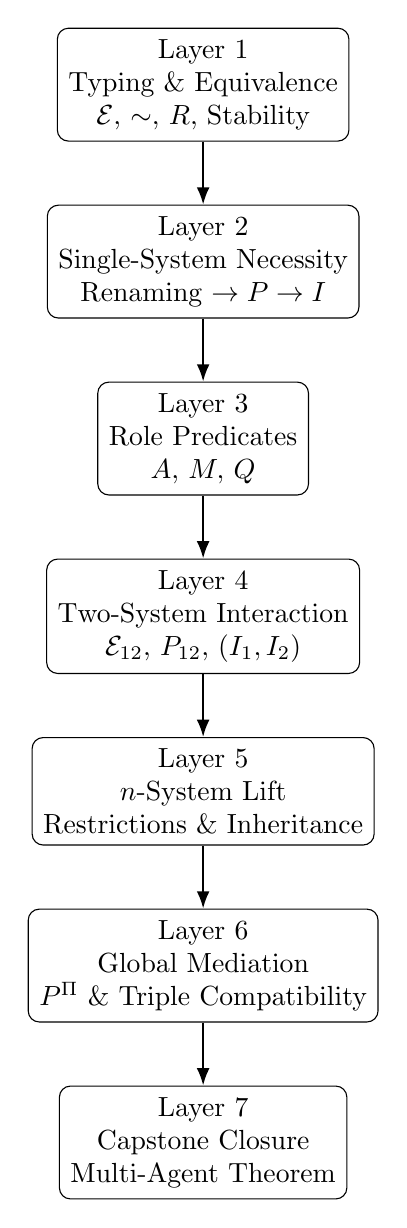
\begin{tikzpicture}[
    node distance=8mm,
    every node/.style={draw, rounded corners, inner sep=4pt, align=center},
    arrow/.style={-{Latex[length=2.2mm]}, thick}
]
\node (L1) {Layer 1\\Typing \& Equivalence\\$\mathcal{E},\,\sim,\,R,$ Stability};
\node (L2) [below=of L1] {Layer 2\\Single-System Necessity\\Renaming $\rightarrow P \rightarrow I$};
\node (L3) [below=of L2] {Layer 3\\Role Predicates\\$A,\,M,\,Q$};
\node (L4) [below=of L3] {Layer 4\\Two-System Interaction\\$\mathcal{E}_{12},\,P_{12},\,(I_1,I_2)$};
\node (L5) [below=of L4] {Layer 5\\$n$-System Lift\\Restrictions \& Inheritance};
\node (L6) [below=of L5] {Layer 6\\Global Mediation\\$P^{\Pi}$ \& Triple Compatibility};
\node (L7) [below=of L6] {Layer 7\\Capstone Closure\\Multi-Agent Theorem};

\draw[arrow] (L1) -- (L2);
\draw[arrow] (L2) -- (L3);
\draw[arrow] (L3) -- (L4);
\draw[arrow] (L4) -- (L5);
\draw[arrow] (L5) -- (L6);
\draw[arrow] (L6) -- (L7);
\end{tikzpicture}
\end{center}

\subsection*{Graph Summary}

Logical flow proceeds strictly upward:

\begin{center}
Typing $\rightarrow$ Stability $\rightarrow$ Mediator/Reference $\rightarrow$
Role Classification $\rightarrow$ Joint Mediation $\rightarrow$
Pairwise Inheritance $\rightarrow$ Global Compatibility $\rightarrow$ Closure
\end{center}

No circular dependencies occur.




\appendix
\section{Core Framework Axioms}

\textbf{A.1 Identity.} $\sim$ permits alpha-equivalence only.

\textbf{A.2 Admissible Redescription.}
Redescription preserves typing, anchors, role assignments, and compatibility.

\textbf{A.3 Redescription Stability.}
\[
R(T(S)) \sim T(R(S)).
\]

\textbf{A.4 Standing.}
Standing is binary, scope-global, conserved, and absorbing.

\textbf{A.5 Non-Triviality.}
Admissibility must attach to conserved structural consequences.

\textbf{A.6 System Boundary Rule.}
All data consulted by a mechanism are part of the system state and must be acted upon by admissible redescriptions.


% ===================== STRUCTURAL HARDENING (INTEGRATED) =====================
\subsection*{Quotient Minimality and Conditional Reference Necessity}
\paragraph{Quotient Universal Property.}
Any redescription-stable evaluation $f:S\to Y$ constant on $\approx$-classes uniquely factors
through the quotient $\pi:S\to S/\approx$. The quotient is therefore the minimal mediator:
any alternative mediator factors through it.

\paragraph{Conditional Reference Necessity.}
If a system assigns \emph{single-valued representatives} in $S$ to quotient states (rather than
working purely in $S/\approx$), then an admissibly invariant section $\kappa:S/\approx\to S$
is required to preserve redescription stability under composition. Absent this condition,
representative choice need not be unique and no invariant resolver is forced.
% ==============================================================================


\paragraph{Irreversibility Scope Note.}
Irreversibility is not required for descent of transitions to the quotient (which follows from stability alone).
It is used only to exclude trivial "repair by backtracking" when discussing single-valued representative selection
and persistence under composition.

\end{document}
